% !TEX encoding = UTF-8 Unicode
% !TEX TS-program = xelatex

\documentclass{article}
	\usepackage[margin = 1.25in]{geometry}
	\usepackage{fontspec}
	\usepackage{tikz}
	\usepackage{listings}
\begin{document}

	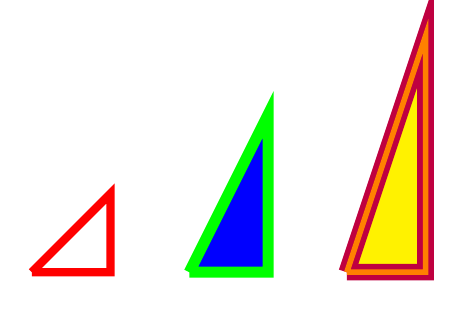
\begin{tikzpicture}
		\draw [red, line width=3pt] (0,0) -- (1,0) -- (1,1) -- (0,0) ;
		\filldraw[fill=blue, draw=green, line width=4]
			(2,0) -- (3,0) -- (3,2) -- (2,0);
		\newcommand\thintriangle{(4,0) -- (5,0) -- (5,3) -- (4,0)}
		\filldraw[fill=yellow, draw=purple, line width=6] \thintriangle;
		\draw    [             draw=orange, line width=2] \thintriangle;
	\end{tikzpicture}

	\fontspec{SourceCodePro-Regular}
	\lstset{
		language=[latex]tex, tabsize=4,
		moredelim=*[s][\itshape]{$}{$},
		moredelim=*[s][\color{red!40!.}]{(}{)},
		moredelim=*[s][\color{green!30!.}]{[}{]},
		backgroundcolor=\color{blue!5},
		commentstyle=\color{.!80}\itshape,
		texcsstyle=*\color{blue!40!.},
		moretexcs={
			draw, filldraw
		},
		deletetexcs={},
	}
	\lstinputlisting{linewidth.tex}

\end{document}